\documentclass[12pt]{article}
\usepackage{graphicx} % Required for inserting images
\usepackage[letter, margin=0.5in]{geometry}
\usepackage{amsmath, mathrsfs, amssymb, cancel} % for various mathematical symbols

\graphicspath{{./images/}}

\setcounter{secnumdepth}{0} % Removes section numbering

\usepackage{titling}
\renewcommand\maketitlehooka{\null\mbox{}\vfill}
\renewcommand\maketitlehookd{\vfill\null}

\title{Physical Mechanics Homework 7}
\date{10/17/2024}
\author{Damien Koon}



\begin{document}

\maketitle

\newpage
\textbf{1. TM 6-3; Show that the shortest distance between two points in three-dimensional
space is a straight line.}

$$
L = \int^{x_2}_{x_1} dS = \int^{x_2}_{x_1} \sqrt{dx^2 + dy^2 + dz^2} = \int^{x_2}_{x_1} \sqrt{\dot{x}^2 + \dot{y}^2 + \dot{z}^2} dt
$$

$$
f(x, \dot{x}, y, \dot{y}, z, \dot{z}, t) = \sqrt{\dot{x}^2 + \dot{y}^2 + \dot{z}^2}
$$

From this functional, three Euler-Lagrange equations will be needed. To satisfy these equations, I will be using $\hat{e}$ in place of $x, y, z$
$$
\frac{\partial f}{\partial \hat{e}} - \frac{d}{dt} \frac{\partial f}{\partial \dot{\hat{e}}} = 0
$$

$$
\frac{\partial f}{\partial \hat{e}} = \frac{\partial}{\partial \hat{e}} \sqrt{\dot{x}^2 + \dot{y}^2 + \dot{z}^2} = 0
$$

$$
\frac{d}{dt} \frac{\partial f}{\partial \dot{\hat{e}}} = 0 \implies \frac{\partial f}{\partial \dot{\hat{e}}} = constant
$$

$$
\frac{\partial f}{\partial \dot{\hat{e}}} = \frac{\partial}{\partial \dot{\hat{e}}} \sqrt{\dot{x}^2 + \dot{y}^2 + \dot{z}^2} = \frac{\dot{\hat{e}}}{\sqrt{\dot{x}^2 + \dot{y}^2 + \dot{z}^2}} = constant
$$

From the previous notation that $\hat{e}$ represents three equations for x, y, z, we will expand it back out to three equations by the radical. 

$$
\frac{\dot{x}}{\sqrt{\dot{x}^2 + \dot{y}^2 + \dot{z}^2}} = C_x \hspace{2cm} 
\frac{\dot{y}}{\sqrt{\dot{x}^2 + \dot{y}^2 + \dot{z}^2}} = C_y \hspace{2cm}
\frac{\dot{z}}{\sqrt{\dot{x}^2 + \dot{y}^2 + \dot{z}^2}} = C_z
$$

For the shortest time length, dt, the radical is equivalent, so these three equations can be equated. 

$$
\frac{\dot{x}}{C_x} = \frac{\dot{y}}{C_y} = \frac{\dot{z}}{C_z}
$$

With some calculus, this simplifies to the equation of a straight line in three dimensions.
$$
\frac{dx}{dt C_x} = \frac{dy}{dt C_y} = \frac{dz}{dt C_z}
$$

$$
\int^{t}_{t_0} \frac{dx}{C_x} dt = \int^{t}_{t_0} \frac{dy}{C_y} dt = \int^{t}_{t_0} \frac{dz}{C_z} dt
$$

$$
(t - t_0)\frac{dx}{C_x} =
(t - t_0)\frac{dy}{C_y} =
(t - t_0)\frac{dz}{C_z}
$$

$$
\int^{x}_{x_0} \frac{dx}{C_x} =
\int^{y}_{y_0} \frac{dy}{C_y} =
\int^{z}_{z_0} \frac{dz}{C_z}
$$


Where the equation of a straight line between three dimensions is represented by:
$$
\boldsymbol{
\frac{x - x_0}{C_x} =
\frac{y - y_0}{C_y} =
\frac{z - z_0}{C_z}
}
$$


\newpage
\textbf{2. TM 6-7; Consider light passing from one medium with index of refraction $n_1$ to another medium with index of refraction $n_2$ (illustrated below for the scenario $n_2 > n_1$). Use Fermat’s Principle—that the travel time is minimized—and derive the law of refraction:}

\centering{$n_1 sin(\theta_1) = n_2 sin(\theta_2)$.}

\centering{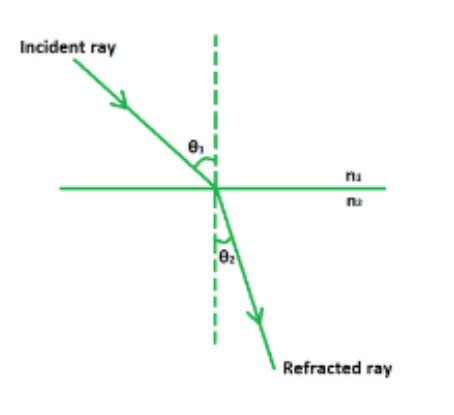
\includegraphics[scale=0.75]{proxy}}

\vspace{1cm}

Let the incident ray begin at the point $(x_1, y_1)$ and end at the point $(0, 0)$
\vspace{0.25cm}

Let the refracted ray begin at the point $(0, 0)$ and end at the point $(x_2, y_2)$ 
\vspace{0.25cm}

Finally, consider a point on the x-axis, $x_c$, such that $x_c$ can be varied to separate the incident and refracted rays by the x-axis
\vspace{0.25cm}

These definitions imply the length of each ray, with the incident ray being denoted $\ell_1$ and the refracted ray being denoted $\ell_2$

$$
\ell_1 = \sqrt{(x_1 - x_c)^2 + (y_1 - 0)^2} 
$$

$$
\ell_2 = \sqrt{(x_2 - x_c)^2 + (y_2)^2} 
$$

From the definition of velocity, the total time it takes to go from the start of the incident ray, $(x_1, y_1)$ to $(x_2, y_2)$ can be found.

$$
v = \frac{x}{t} \implies t = \frac{x}{v} \implies t_{tot} = \frac{\ell_1}{v_1} + \frac{\ell_2}{v_2}
$$

The speed at which light takes to travel from the start of the medium defined above and below the x-axis is equal to the index of refraction, n divided by the speed of light.

$$
v = \frac{c}{n} \implies t_{tot} = \frac{n_1 \ell_1}{c} + \frac{n_2 \ell_2}{c}
$$

\newpage

We want to minimize the total time, so that would imply

$$
\frac{dt}{d x_c} = 0
$$

$$
\frac{d}{d x_c} ( \frac{n_1 \ell_1}{c} + \frac{n_2 \ell_2}{c} ) = 0
$$

To further reduce the equation, the speed of light can be factored out

$$
\frac{d}{d x_c} ( n_ 1 \sqrt{(x_1 - x_c)^2 + (y_1)^2} + n_ 2 \sqrt{(x_2 - x_c)^2 + (y_2)^2} ) = 0
$$

After applying the chain rule, the two parts of the equation can be given as:
$$
n_1(\frac{1}{2} \frac{-2 (x_1 - x_c)}{\sqrt{(x_1 - x_c)^2 + (y_1)^2}})  + n_2(\frac{1}{2} \frac{-2 (x_2 - x_c)}{\sqrt{(x_2 - x_c)^2 + (y_2)^2}}) = 0
$$

Which then reduces to:
$$
n_1(\frac{x_1 - x_c}{\sqrt{(x_1 - x_c)^2 + (y_1)^2}}) = n_2(\frac{x_2 - x_c}{\sqrt{(x_2 - x_c)^2 + (y_2)^2}})
$$

The parts of the equation in the parenthesis are the definition of sine, which then after reductionl becomes Snell's law.

$$
\boldsymbol{
n_1 sin(\theta_1) = n_2 sin(\theta_2)
}
$$

\end{document}